\documentclass[
    a4paper,
    11pt,
    oneside,
    numbers=noendperiod,
    abstract=true
]{scrartcl}

\usepackage[a4paper,margin=2.5cm]{geometry}

\usepackage{microtype}
\usepackage{graphicx}
\usepackage{amsmath,amssymb}
\usepackage{booktabs}
\usepackage{siunitx}
\usepackage{csquotes}
\usepackage[version=4]{mhchem}

\usepackage[
    backend=biber,
    style=numeric,
    sorting=none,
    maxnames=3,
    minnames=1
]{biblatex}
\addbibresource{references.bib}

\usepackage{hyperref}
\usepackage[nameinlink,noabbrev]{cleveref}

\graphicspath{{figures/}}

\sisetup{group-minimum-digits=4, group-digits=integer}

%Let floats share a page with text instead of collecting onto float-only pages
\renewcommand{\topfraction}{0.88}
\renewcommand{\bottomfraction}{0.7}
\renewcommand{\textfraction}{0.1}
\renewcommand{\floatpagefraction}{0.8}

\newcommand{\Rsq}{$R^2$}

\begin{document}

\begin{titlepage}
    \centering
    {\Large University of Copenhagen / Department of Computer Science\par}
    \vspace{2cm}

    {\Huge\bfseries Analyzing Greenland's Geochemistry through Machine Learning\par}
    \vspace{1.5cm}

    {\Large Research Project Report\par}
    \vfill

    {\large
    Salvador Wahnon Palma\\
    Supervisor: Bulat Ibragimov\\
    \today
    \par}
\end{titlepage}

\begin{abstract}
Greenland is among the world's most mineral-rich but least-explored regions, and the Geological
Survey of Denmark and Greenland (GEUS) publishes decades of geochemical sampling as open data.
This report asks whether a held-out element can be predicted from a sample's remaining elements,
and whether knowing \emph{where} the sample came from helps. One pipeline is applied unchanged
to two independent GEUS datasets with deliberately different sampling geometries: whole-rock
geochemistry (\num{6957} samples, clustered along the West Greenland margin) and stream sediment
(\num{17463} samples, spanning the whole ice-free coast).

Own chemistry predicts a held-out element well, reaching a mean \Rsq{} of \num{0.868} on stream
sediment and \num{0.798} on whole rock over 71 and 48 target elements. Spatial context adds
little on top: neighbouring chemistry, three full-coverage geophysical grids and raw coordinates
each contribute less than one fold standard deviation, and are largely interchangeable with one
another. A graph neural network with learned, distance-weighted aggregation does not beat a
hand-specified average over the same neighbourhood.

The gain is not uniform, and its structure is the main result. Stratifying targets by how well
own chemistry already predicts them gives a clean monotone decay --- roughly $+0.05$ \Rsq{}
where chemistry fails, nothing where it already exceeds \num{0.95} --- and the curve reproduces
across both datasets despite their different geometries and target sets. The elements that
benefit form a coherent group: the hydrothermal pathfinder suite (As, Sb, Pb, Cs on both
datasets) led by uranium on stream sediment, which rises from \num{0.594} to \num{0.814}.
Measuring the chemistry directly identifies what those elements share --- they are the ones with
no close companion element in the same sample, so nothing local substitutes for the target. All
results use random $k$-fold cross-validation; spatially blocked evaluation, where these
conclusions are most exposed, is set out as the next stage.
\end{abstract}

\tableofcontents

\section{Introduction}
\label{ch:introduction}

Since the 1950s, government surveys and exploration companies have sampled rock outcrops and
stream catchments along Greenland's ice-free margin. The resulting analyses --- \num{46226} rows
of them in the two datasets used here --- are published by GEUS through the Greenland Mineral
Resources Portal \parencite{greenland_portal}.

The archive is attractive to machine learning for the same reasons it is awkward. Coverage is
heterogeneous: some outcrops carry dozens of samples while entire regions carry none. Analytical
suites differ by campaign, so the element matrix is sparse and its sparsity is not random.
Concentrations are compositional and span six orders of magnitude, from weight percent to parts
per billion. And everything is spatially autocorrelated, because neighbouring catchments drain
the same lithologies \parencite{tobler1970} --- which is at once the motivation for spatial
modelling and the main threat to evaluating it honestly.

\subsection{Research questions}

The project was organised around three questions agreed with the supervisor.

\begin{description}
    \item[RQ0 --- report parsing.] Convert scanned exploration reports into structured records
        with a public language model. \emph{Dropped by agreement:} the scans rarely contain the
        assay tables that would make parsing useful, and the geochemical database is already
        available in structured form.
    \item[RQ1 --- missing geochemistry.] Given a sample with some elements measured, predict a
        held-out element from (a) the sample's other elements and (b) its spatial neighbourhood.
        \emph{This report.}
    \item[RQ2 --- unexplored regions.] Predict concentrations in a geological area held out
        \emph{spatially} rather than at random. This is regression under spatial hold-out, not
        prospectivity classification. \emph{Scoped and prepared; see \Cref{ch:conclusion}.}
\end{description}

\subsection{Contributions}

One pipeline is applied unchanged to two GEUS datasets with markedly different sampling
geometries, so every claim below can be checked for dataset-specificity rather than asserted
from one. On that footing the report contributes: a comparison of four ways of encoding a
spatial neighbourhood as tabular features, across seven neighbourhood sizes and two model
families, showing that a neighbourhood should be \emph{pooled} rather than \emph{enumerated};
evidence that spatial context --- as neighbouring chemistry, geophysical grids, raw coordinates,
or a learned graph aggregation --- is largely redundant with a sample's own chemistry, together
with a direct measurement of why, and of which elements escape it; and a graph neural network
evaluated against the hand-built encodings on identical folds, including whether edge distance
carries information a fixed-radius average cannot express. It does not.

\section{Data and method}
\label{ch:method}

\subsection{Two datasets}
\label{sec:datasets}

Two public GEUS geochemistry datasets are used, both processed by the same code. They were
chosen because they differ sharply in sampling geometry (\Cref{fig:samples,tab:datasets}). Whole
rock is clustered exploration sampling within a narrow band of West Greenland; stream sediment
covers the entire ice-free margin with a fifth of the co-location. If a conclusion depends on
how a survey was laid out, these two should disagree.

\begin{figure}[htbp]
\centering
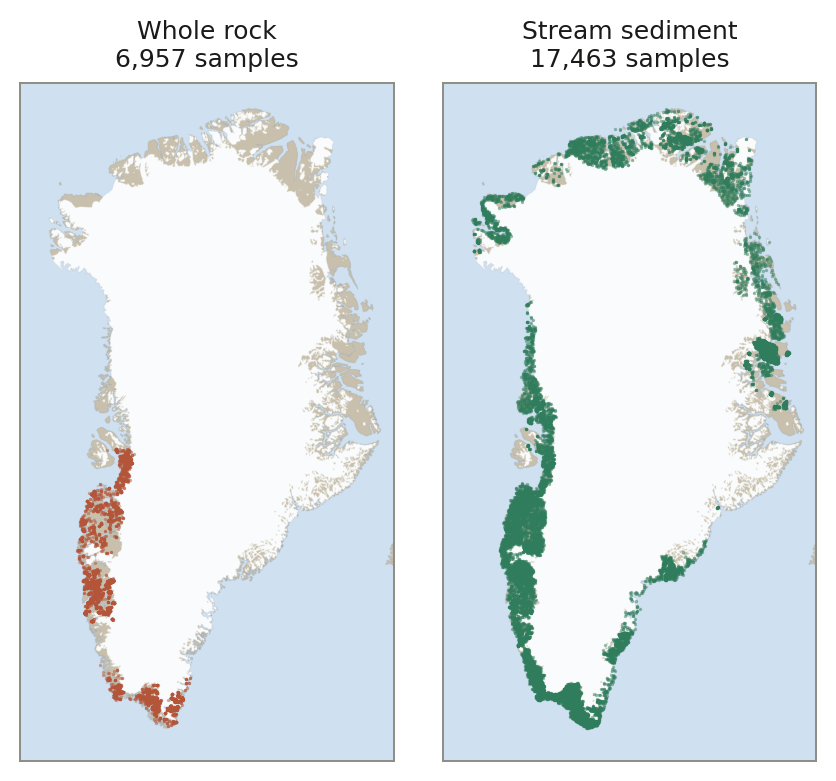
\includegraphics[width=0.50\textwidth]{samples.png}
\caption[Sample locations]{Sample locations after preprocessing. Whole rock is confined to one
region of the west coast; stream sediment follows the whole ice-free margin, including the far
north and east.}
\label{fig:samples}
\end{figure}

\begin{table}[htbp]
\centering
\caption[The two GEUS datasets]{The two datasets, before and after preprocessing.}
\label{tab:datasets}
\begin{tabular}{lrr}
\toprule
 & Whole rock & Stream sediment \\
\midrule
Raw rows                       & \num{26068}   & \num{20158} \\
Raw element columns            & 76            & 523 \\
Merged physical samples        & \num{6957}    & \num{17463} \\
Element columns after merging  & 76            & 93 \\
Target elements (coverage $\geq$ \num{1000}) & 48 & 71 \\
\midrule
Unique coordinate pairs        & \num{4498}    & \num{16542} \\
Samples sharing a coordinate   & \num{3458} (50\,\%) & \num{1759} (10\,\%) \\
Maximum samples at one coordinate & 67         & 11 \\
Longitude span                 & \ang{11.7}    & \ang{59.5} \\
\bottomrule
\end{tabular}
\end{table}

Stream sediment's 523 raw element columns are 93 elements each measured by up to four
laboratory and method combinations (for instance \texttt{ACTLABS FUS ICP Ni ppm} alongside
\texttt{ACTLABS INAA Ni ppm}); whole rock already carries one column per element. Co-location is
genuine sampling density rather than duplication --- 67 samples at one outcrop reflects a
detailed campaign --- so it is retained in both datasets, and its effect is instead controlled
for at feature-construction time (\Cref{sec:neighbours}).

Each source file carries a schema in JSON naming the sample identifier, metadata, physical and
location columns; element columns are whatever remains. Longitude and latitude are classified as
metadata, so coordinates never enter the chemistry feature set by accident.

\subsection{Preprocessing}
\label{sec:pipeline}

Six steps, whose order is load-bearing:

\begin{enumerate}
    \item \textbf{Mask below-detection values.} Entries $\leq 0$ encode ``below detection limit''
        and become missing --- an analysis that finds nothing reports a sentinel, not a zero.
        Done \emph{first}, so a negative reading can never contaminate a median computed later.
    \item \textbf{Merge analytical columns.} Per-laboratory, per-method columns of one element
        collapse to one, by median across whichever methods measured that sample. Methods differ
        in detection limit and bias, so the median is the neutral choice rather than an obvious
        one. Stream sediment goes from 523 columns to 93; whole rock is untouched.
    \item \textbf{Merge by sample number.} Median across duplicate rows describing one physical
        sample.
    \item \textbf{Log-transform.} Base-10, after both merges, so the result is a log of medians
        rather than a median of logs. Concentrations spanning weight percent to parts per billion
        are otherwise incomparable across elements \parencite{aitchison1982}.
    \item \textbf{Coverage filter.} Element columns measured in fewer than 10 samples are
        dropped. Last on purpose: filtering earlier would discard measurements the two merges
        would have rescued.
    \item \textbf{Splits.} An 80/10/10 holdout and a five-fold random cross-validation
        assignment, both written to disk so every experiment sees identical folds.
\end{enumerate}

\subsection{Targets and evaluation}
\label{sec:evaluation}

Every element measured in at least \num{1000} samples is a target: 48 on whole rock, 71 on
stream sediment. A coverage threshold is preferred to the more usual ``$n$ best-covered
elements'' because it does not depend on how many elements a dataset happens to contain;
\Cref{sec:targetsensitivity} shows that this choice materially changes the headline number.

Each target is predicted from the sample's remaining elements, scored by \Rsq{} on the
log-transformed scale over five random folds, and only on samples where that target was actually
measured. Tables report the mean over target elements.

Because a mean over dozens of elements hides a great deal, the standard deviation across folds,
averaged over elements, is used as a noise floor: \num{0.0180} on whole rock and \num{0.0137} on
stream sediment. Differences smaller than this are not interpreted as real, and are quoted in
units of it where the comparison matters.

\textbf{All folds are random.} Under random cross-validation a test sample frequently has
training samples a few hundred metres away, so a model can appear to generalise spatially while
in fact interpolating between near-duplicates \parencite{roberts2017}. Spatial blocking is RQ2
and is deliberately not conflated with these results; \Cref{sec:limitations} states which
conclusions are expected to be sensitive to it.

\subsection{Encoding a neighbourhood}
\label{sec:neighbours}

Neighbour features are built at training time, per fold. A $k$-d tree is fitted on
\emph{training coordinates only} and queried with all rows, so a test sample can never see
another test sample; self-matches are pushed to infinite distance. Distance-zero neighbours are
additionally discarded throughout, which separates ``another sample from the same outcrop'' from
``a genuinely different place'' --- without this control, half the whole-rock dataset would draw
its neighbourhood from its own sampling site.

Four encodings of that neighbourhood are compared. With $k$ neighbours and $m$ elements they
differ in how much they aggregate (\Cref{tab:encodings}), and the contrast between the pooled
variants and the enumerated one is the point of the comparison.

\begin{table}[htbp]
\centering
\caption[The four neighbour encodings]{The four neighbour encodings. Column counts are for
$k=20$, $m=87$ (stream sediment). Only variant~C has a width independent of $k$.}
\label{tab:encodings}
\begin{tabular}{clr}
\toprule
Variant & Content & Added columns \\
\midrule
A & Mean of the \emph{target} element over $k$ neighbours & 1 \\
B & The $k$ individual \emph{target} values               & 20 \\
C & Mean of \emph{every} element over $k$ neighbours      & 87 \\
D & \emph{Every} element of \emph{every} neighbour        & \num{1740} \\
\bottomrule
\end{tabular}
\end{table}

\subsection{Geophysical grids}
\label{sec:geophysics}

Geochemical neighbours only exist where somebody has already sampled; geophysical grids are
measured everywhere. They are therefore the natural substitute for a neighbourhood on
unexplored ground, and the geologically motivated input the project set out to add.

Three grids qualified on the criterion of \emph{complete Greenland coverage}, assessed over the
whole landmass rather than over the samples at hand: magnetic anomaly \parencite{geus_greenmag},
which tracks how magnetite-rich the underlying rock is; geothermal heat flow
\parencite{geus_heatflow}, which reflects tectonic setting and the decay of U, Th and K; and
depth to Moho \parencite{geus_moho}, which is crustal thickness --- thin under rifted margins,
thick under old craton. All three are valid at 100\,\% of samples in both datasets. They are
attached before the splits, since they are static per coordinate and carry no train/test
dependence.

Candidate gravity products were rejected on a criterion worth stating, because it is invisible
from the files: North Atlantic compilations contain no missing values over Greenland only
because they contain no measurement \emph{points} over its west, at a median
\SI{157}{\kilo\metre} from a sample to the nearest grid node. Absence of \texttt{NaN} is not
evidence of coverage.

\subsection{Models}
\label{sec:models}

Gradient-boosted decision trees remain the strongest general-purpose learners on tabular data of
this size and heterogeneity \parencite{grinsztajn2022}. The main model is the histogram-based
gradient boosting implementation in scikit-learn \parencite{pedregosa2011}, which follows the
binning strategy of LightGBM \parencite{ke2017lightgbm}: features are discretised before splits
are searched, which makes training near-linear in sample count and handles missing values
natively --- essential here, since the element matrix is sparse by construction. A random forest
\parencite{breiman2001} and XGBoost \parencite{chen2016xgboost} are run as comparison points
(\Cref{sec:baseline}), and the random forest is retained as an independent check that
conclusions are not an artefact of one inductive bias (\Cref{sec:robustness}).

\subsection{Graph neural network}
\label{sec:gnnmethod}

A graph model offers a different way to use a neighbourhood: rather than summarising it into
fixed columns, it learns an aggregation over a graph. Here the graph has one node per sample and
directed edges from each of a sample's $k$ nearest \emph{training} neighbours --- exactly the
mapping the tabular encodings use, so the network sees the same neighbourhood the hand-built
columns saw. Each edge carries $\log(1+d)$, with $d$ in kilometres, as its feature.

Node features are the sample's own elements with the target removed. Because a network cannot
consume a missing value, each element contributes two channels: the standardised value, zeroed
where absent, and a present/absent flag, so the model can distinguish ``average'' from ``not
measured''. Standardisation statistics come from training rows only.

Two architectures are compared, and the contrast is the experiment.
\textsc{GraphSAGE} \parencite{hamilton2017} aggregates neighbours with a permutation-invariant
operator and is distance-blind by construction. A graph attention network
\parencite{velickovic2018} with \texttt{edge\_dim=1} instead computes attention weights per edge
\emph{from the distance}, which is the one thing variants A--D structurally cannot encode. Both
use two message-passing layers of hidden width 64, a skip connection carrying the node's own
features to a two-layer head, dropout \num{0.1}, and Adam at learning rate $10^{-2}$ with weight
decay $10^{-4}$. Training is full-batch and transductive: the whole graph is passed forward each
epoch, but the loss only ever sees training nodes, and the stopping epoch is chosen on a
validation slice carved out of the \emph{training} nodes. Implementation uses PyTorch Geometric
\parencite{fey2019}; runs took approximately \SI{9.1}{\second} per fit at $k=20$ on a Colab T4.

Graph experiments were run on stream sediment, the dataset where standalone spatial signal is
strong enough (\Cref{sec:featuresets}) for a learned aggregation to have something to compete
over.

\section{Results}
\label{ch:results}

\subsection{Own chemistry sets a high baseline}
\label{sec:baseline}

Predicting a held-out element from a sample's remaining elements reaches a mean \Rsq{} of
\num{0.7983} on whole rock (48 targets) and \num{0.8676} on stream sediment (71 targets). This
is the number every spatial method below must improve upon, and it is high because elements are
strongly co-determined: a sample rich in \ce{SiO2} is necessarily poor in something else.

The two figures are not directly comparable to one another, since the target sets differ ---
whole rock's 48 elements are proportionally more trace metals, stream sediment's 71 include a
large suite of near-collinear rare earths that are easy to predict. Every comparison in this
chapter is therefore made \emph{within} a dataset.

Among the three tabular learners, gradient boosting was both the most accurate --- on every one
of the ten whole-rock elements tested --- and the fastest, at mean \Rsq{}~\num{0.8388} in
\SI{155}{\second} against \num{0.8207} in \SI{388}{\second} for a 200-tree random forest and
\num{0.8215} in \SI{199}{\second} for XGBoost. It is used throughout. XGBoost's tie with the
random forest is consistent with its competitive reputation resting on extensive tuning that its
defaults (\texttt{max\_depth}~$=6$, \texttt{learning\_rate}~$=0.3$) do not supply for a dataset
of this size and correlation structure.

\subsection{A neighbourhood should be pooled, not enumerated}
\label{sec:variants}

\Cref{tab:variants} gives the four encodings at $k=20$. The shape is the same on both datasets:
variant~C is best, variant~D lands at or below the baseline, and every gain is smaller than one
fold standard deviation --- $0.82\sigma$ on whole rock, $0.91\sigma$ on stream sediment.

\begin{table}[htbp]
\centering
\caption[Neighbour encodings on both datasets]{The four neighbour encodings, $k=20$, co-located
neighbours excluded. Fold standard deviation is \num{0.0180} (whole rock) and \num{0.0137}
(stream sediment).}
\label{tab:variants}
\begin{tabular}{lrrrr}
\toprule
 & \multicolumn{2}{c}{Whole rock (48)} & \multicolumn{2}{c}{Stream sediment (71)} \\
\cmidrule(lr){2-3}\cmidrule(lr){4-5}
Variant & Mean \Rsq{} & $\Delta$ & Mean \Rsq{} & $\Delta$ \\
\midrule
Baseline (no neighbours) & \num{0.7983} & ---            & \num{0.8676} & --- \\
A                        & \num{0.8043} & $+0.0059$      & \num{0.8757} & $+0.0081$ \\
B                        & \num{0.8050} & $+0.0066$      & \num{0.8724} & $+0.0048$ \\
\textbf{C}               & \textbf{\num{0.8132}} & $\mathbf{+0.0149}$ & \textbf{\num{0.8801}} & $\mathbf{+0.0125}$ \\
D                        & \num{0.7982} & $-0.0001$      & \num{0.8659} & $-0.0017$ \\
\bottomrule
\end{tabular}
\end{table}

Sweeping $k$ from 1 to 100 (\Cref{fig:ksweep}) separates aggregation from dimensionality, and
two trends run in opposite directions on both datasets. Variant~C improves with $k$ and plateaus
around $k \approx 20$--$50$: because it averages over the neighbourhood, its width stays at $m$
columns whatever $k$ is, so more neighbours only smooth sampling noise and cost nothing.
Variant~D degrades monotonically, and the decline tracks its column count exactly --- \num{1740}
columns at $k=20$, \num{8700} at $k=100$. D contains strictly more information than C and uses
it strictly worse.

\begin{figure}[htbp]
\centering
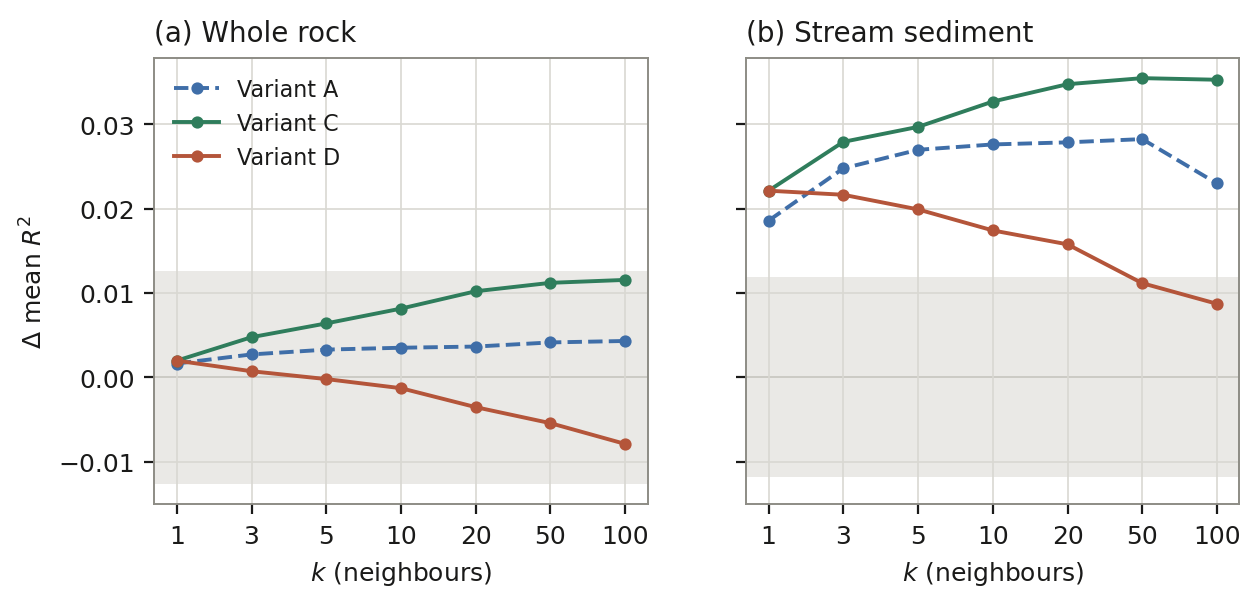
\includegraphics[width=0.92\textwidth]{ksweep.png}
\caption[Neighbour encodings across $k$]{Change in mean \Rsq{} over the no-neighbour baseline as
neighbourhood size $k$ varies, on the ten best-covered elements of each dataset. The grey band
is one fold standard deviation. Variant~C (pooled) rises and plateaus; variant~D (enumerated)
falls in step with its column count. Absolute levels reflect the ten-element target sets
(\Cref{sec:targetsensitivity}); the shape is what this figure establishes.}
\label{fig:ksweep}
\end{figure}

This is the most robust result in the report --- it holds across two datasets, two model
families and seven values of $k$ --- and it fixes $k=20$ for everything that follows: the onset
of the plateau, and effectively free for variant~C, whose column count does not depend on $k$.

\subsection{Where the gain lands}
\label{sec:difficulty}

A pooled mean over dozens of elements averages together very different behaviours. Binning
targets by \emph{their own baseline score} separates the elements own chemistry already predicts
from those it cannot (\Cref{fig:difficulty}).

\begin{figure}[htbp]
\centering
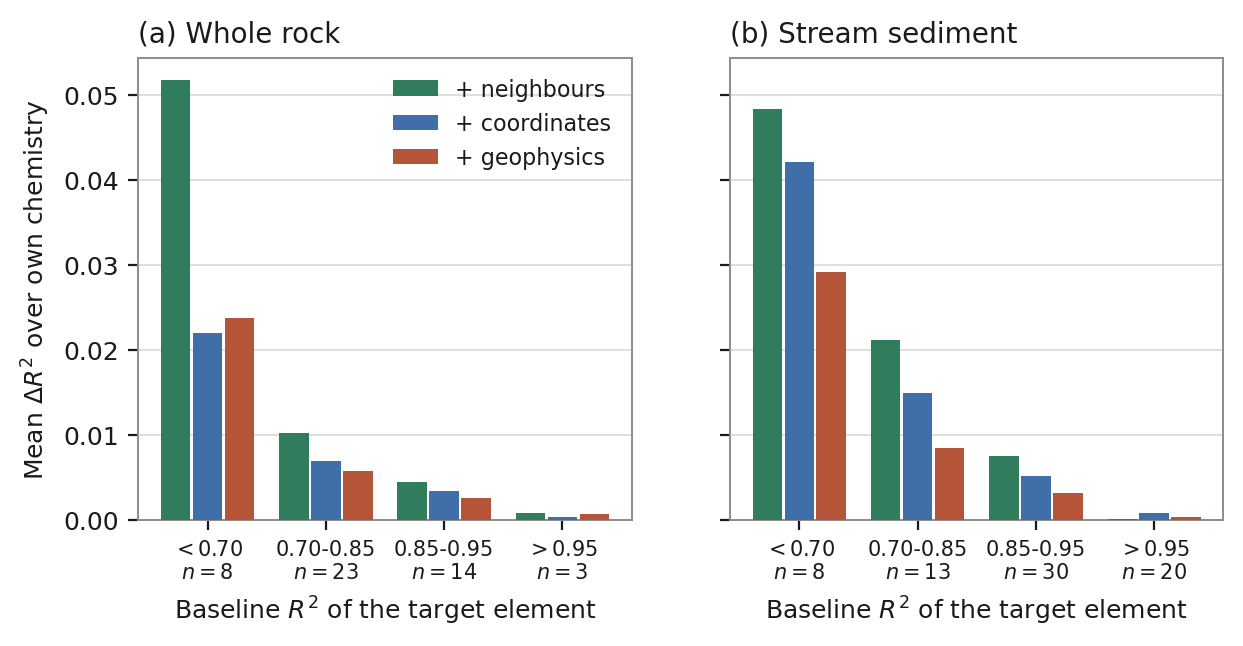
\includegraphics[width=0.92\textwidth]{difficulty.png}
\caption[Gain stratified by baseline difficulty]{Mean improvement over own chemistry, with
targets grouped by how well own chemistry already predicts them. Two datasets with different
sampling geometries, different target sets and different element counts produce almost the same
curve.}
\label{fig:difficulty}
\end{figure}

The decay is monotone on both datasets and the two curves are nearly identical, despite the
datasets differing in sample count, spatial extent, co-location rate and target composition.
Neighbours are worth $+0.0517$ to the eight whole-rock targets below \num{0.70} (mean baseline
\num{0.5920}) and $+0.0484$ to the eight stream-sediment ones (\num{0.5846}); above \num{0.95}
they are worth $+0.0008$ across three whole-rock targets and $+0.0001$ across twenty stream ones
--- unsurprisingly, since there is no headroom left to fill. \textbf{This, rather than any
pooled mean, is the central result of RQ1}, and it explains mechanically why a pooled mean is
fragile: changing the target set changes the mixture of difficulty bands, and therefore the
average, without anything about the underlying behaviour changing at all.

\subsection{Which elements benefit}
\label{sec:pathfinders}

The elements gaining most are not an arbitrary assortment, and they recur across the two
datasets (\Cref{tab:pathfinders}). Arsenic, antimony, lead and caesium appear in both top-six
lists, computed on different samples, different target sets and different sampling geometries.

\begin{table}[htbp]
\centering
\caption[Elements with the largest neighbour gain]{The six elements with the largest gain from
neighbour features on each dataset, $k=20$. Four elements (As, Sb, Pb, Cs) appear on both lists.}
\label{tab:pathfinders}
\begin{tabular}{lrlr}
\toprule
\multicolumn{2}{c}{Whole rock} & \multicolumn{2}{c}{Stream sediment} \\
\cmidrule(lr){1-2}\cmidrule(lr){3-4}
Element & $\Delta$ \Rsq{} & Element & $\Delta$ \Rsq{} \\
\midrule
As & $+0.096$ & U  & $\mathbf{+0.220}$ \\
Au & $+0.092$ & As & $+0.060$ \\
Sb & $+0.070$ & Br & $+0.043$ \\
Cs & $+0.048$ & Sb & $+0.041$ \\
S  & $+0.040$ & Pb & $+0.034$ \\
Pb & $+0.027$ & Cs & $+0.031$ \\
\bottomrule
\end{tabular}
\end{table}

These are, bromine aside, the classical hydrothermal pathfinder suite together with mobile
alkalis: elements whose distribution is governed by regional-scale processes such as
mineralisation and alteration rather than by bulk rock composition, and which therefore have
something for a neighbourhood to say that the host rock's major elements do not. Uranium is the
extreme case, rising on stream sediment from \num{0.594} on own chemistry alone to \num{0.814}
with neighbours. It is also the only element with a reliable geophysical correlation in this
data ($+0.28$ with magnetic anomaly, $-0.34$ with Moho depth, $n=\num{3227}$), which is coherent
--- uranium concentrates in evolved felsic crust, which is thick and weakly magnetic.

\subsection{Chemical isolation is the common cause}
\label{sec:isolation}

\Cref{sec:difficulty,sec:pathfinders} give two descriptions of the same set of elements --- ones
own chemistry predicts poorly, and ones that are geochemically mobile --- which invites the
question of what the two have in common. Measuring the chemistry directly answers it. For each
element, take the single strongest Spearman correlation it has with any other element in the same
sample, computed pairwise-complete over the raw log concentrations and independently of any model.
Call that its \emph{companion strength}: how good a proxy the sample already carries.

\begin{figure}[htbp]
\centering
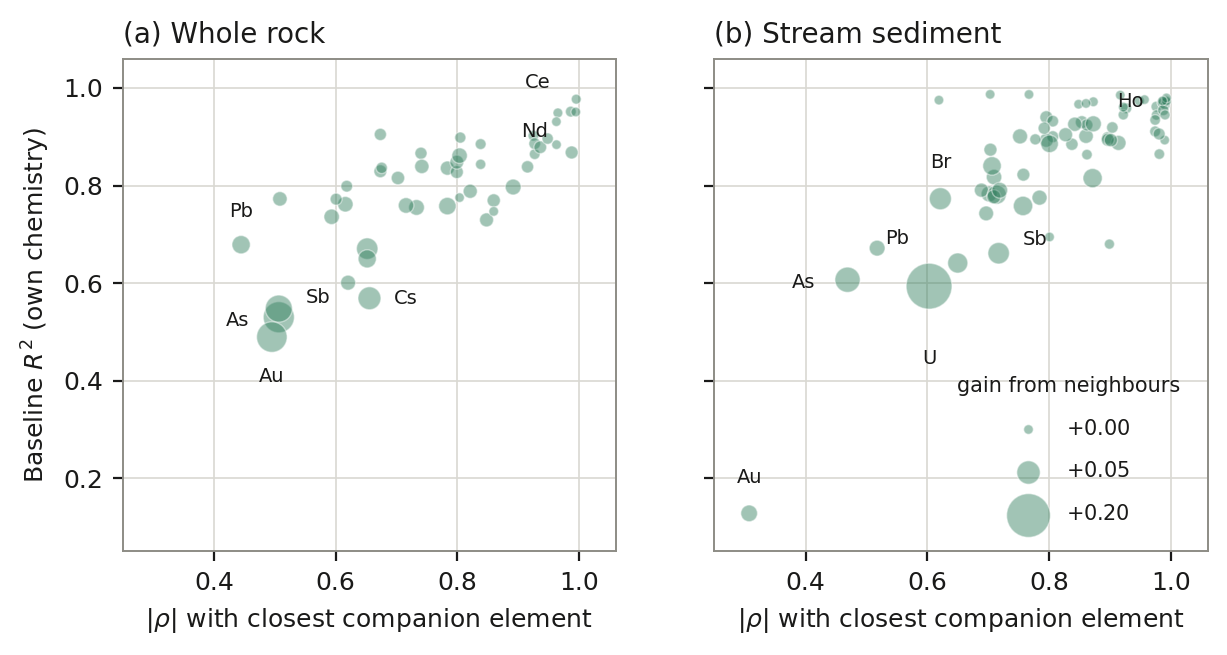
\includegraphics[width=0.92\textwidth]{isolation.png}
\caption[Chemical isolation]{Baseline \Rsq{} against companion strength, one point per target
element; marker area is the gain from neighbour features. Elements with a near-perfect companion
sit top right and gain nothing; chemically isolated elements sit lower left and are where the
neighbourhood pays. Uranium is the extreme case on stream sediment.}
\label{fig:isolation}
\end{figure}

Companion strength predicts the baseline on both datasets ($r=+0.77$ and $+0.76$), and predicts
the neighbour gain with the opposite sign (Spearman $-0.70$ and $-0.63$). Splitting targets on
whether they have any partner above $\rho=0.8$ separates them cleanly, and the two datasets
agree despite sharing neither target set nor sampling geometry: elements with such a partner
average a baseline of \num{0.864} on whole rock and \num{0.920} on stream sediment and gain
$+0.0047$ from neighbours on both, while chemically isolated elements average \num{0.738} and
\num{0.782} and gain $+0.0242$ and $+0.0253$ --- five times as much, on roughly half the targets
in each dataset.

The mechanism this exposes is a substitution. The elements at the top right are the rare earths,
which track one another almost perfectly (Ce--Pr $\rho = \num{0.995}$, Ho--Er $\rho = \num{0.993}$)
and are therefore predictable from a single companion in the same sample; a neighbourhood tells
such an element nothing it does not already know. The elements at the lower left have no proxy at
all: gold's best companion is $\rho = \num{0.31}$ on stream sediment, uranium's $\num{0.60}$,
arsenic's $\num{0.47}$, and none of the three has a single partner above $\num{0.8}$.
\textbf{Spatial context is worth something precisely where the sample's own chemistry contains no
substitute for the target.}

This also unifies the two readings of \Cref{sec:pathfinders}. ``Mobile element'' and ``hard
target'' are not competing explanations but the same one seen from either side: an element whose
concentration is set by mineralisation or alteration rather than by bulk composition is, for that
reason, one that nothing else in the sample tracks --- which makes it both hard to predict and
responsive to where it was found. The confound noted in \Cref{sec:limitations} is not removed by
this, since isolation still explains both, but it is named.

\subsection{Where the spatial information comes from}
\label{sec:featuresets}

Scoring each feature source alone and in combination (\Cref{fig:featuresets}) splits the
question in two, and the two halves answer differently.

\begin{figure}[htbp]
\centering
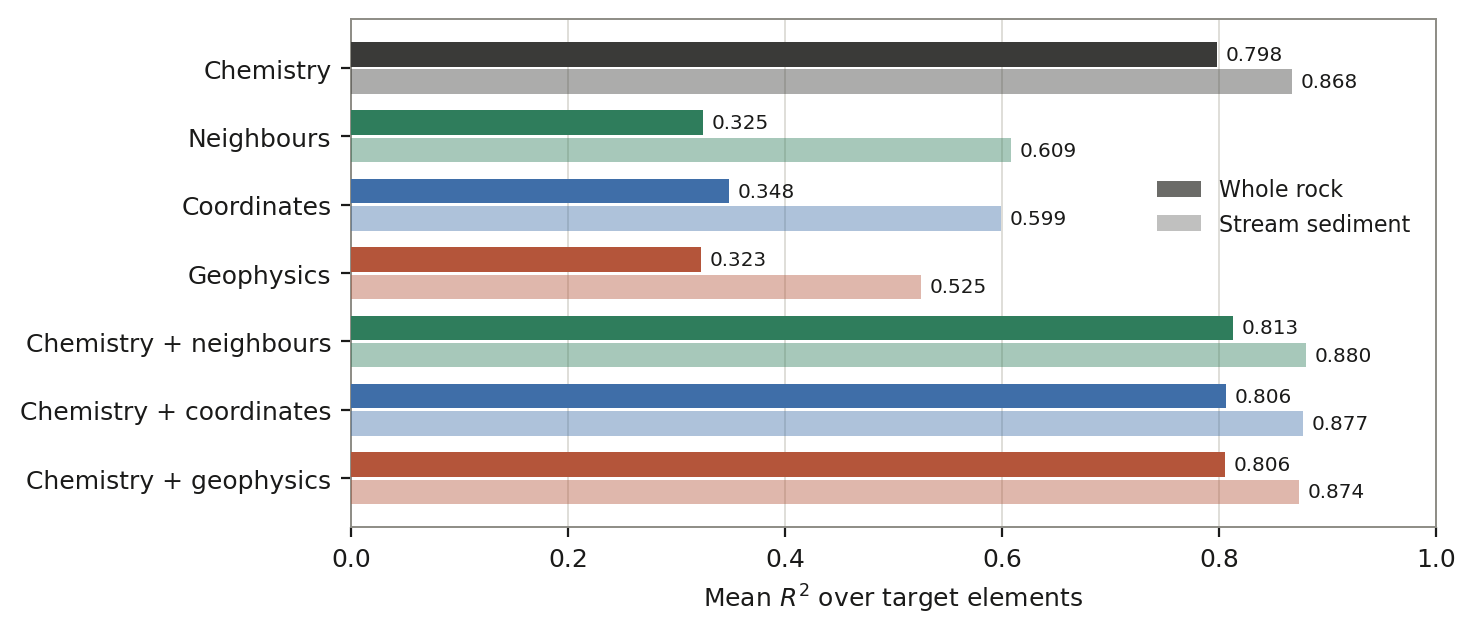
\includegraphics[width=0.88\textwidth]{featuresets.png}
\caption[Feature-source ablation]{Mean \Rsq{} by feature source, coverage-threshold target sets.
Colour identifies the feature source, opacity the dataset. The upper block (spatial information
alone) roughly doubles from whole rock to stream sediment; the lower block (the same information
on top of own chemistry) barely moves.}
\label{fig:featuresets}
\end{figure}

\paragraph{Sampling geometry decides how much spatial information exists.} Every standalone
spatial source is roughly twice as informative on stream sediment as on whole rock: neighbours
\num{0.325} against \num{0.609}, coordinates \num{0.348} against \num{0.599}, geophysics
\num{0.323} against \num{0.525}. This is a large and robust difference, and exactly what the
dispersed-versus-clustered contrast of \Cref{fig:samples} would predict.

\paragraph{It does not decide how much that information adds.} Five times the standalone spatial
signal buys the same sub-$\sigma$ improvement on top of own chemistry: $+0.0149$ against
$+0.0125$ for neighbours, $+0.0080$ against $+0.0099$ for coordinates, $+0.0076$ against
$+0.0063$ for geophysics. The reason is redundancy --- a sample's own chemistry already encodes
most of what its location would tell you, because chemistry is what location predicts.

\paragraph{The three spatial sources are interchangeable.} Geophysics, coordinates and
neighbours land in one narrow band on each dataset, and each adds between $+0.006$ and $+0.015$
on top of chemistry. In particular \textbf{the geophysical grids do not beat plain coordinates}:
coordinates outscore geophysics on both datasets, and combining the two barely exceeds
coordinates alone (\num{0.6017} against \num{0.5994} on stream sediment). On this evidence the
grids encode \emph{where} a sample is rather than independently \emph{what} lies underneath it.

A correlation test outside the models agrees. Comparing, for each element, its strongest
correlation with a geophysical field against its strongest correlation with raw easting or
northing, geophysics wins for only 27 of 64 elements (42\,\%) on whole rock and 26 of 81 (32\,\%)
on stream sediment. How far a grid is a position proxy depends on the sampling footprint rather
than on the grid: depth to Moho correlates $r = \num{0.75}$ with northing across whole rock's
narrow longitude band, but only $-\num{0.23}$ across stream sediment's full-island coverage.
\Cref{sec:limitations} explains why this is the reading most likely to invert under spatial
cross-validation.

\subsection{A learned aggregation does not do better}
\label{sec:gnnresults}

\Cref{fig:gnn} compares both graph architectures against variant~C across the same seven values
of $k$, on identical folds.

\begin{figure}[htbp]
\centering
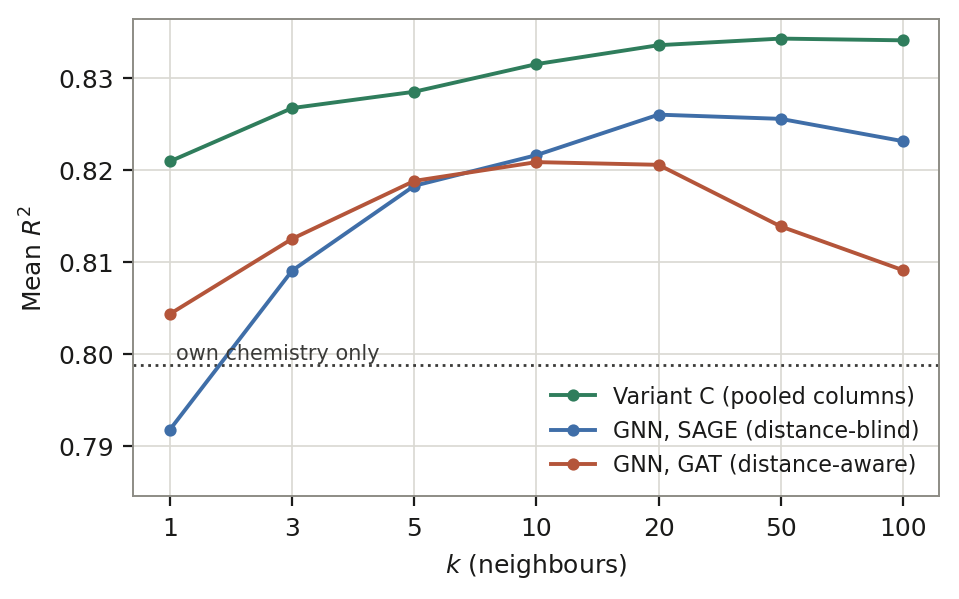
\includegraphics[width=0.62\textwidth]{gnn.png}
\caption[Graph networks against hand-built neighbour features]{Mean \Rsq{} on stream sediment for
the two graph architectures and the hand-built pooled encoding, across neighbourhood size.
Variant~C dominates both networks at every $k$. Distance-aware attention (GAT) beats the
distance-blind control (SAGE) only below $k \approx 5$, and degrades above $k=20$.}
\label{fig:gnn}
\end{figure}

\paragraph{The hand-built encoding wins everywhere.} Variant~C is above both networks at all
seven values of $k$, with no crossover. The best network is \textsc{GraphSAGE} at $k=20$
(\num{0.8260}); the best hand-built result is variant~C at $k=50$ (\num{0.8342}).

\paragraph{Distance-aware attention does not pay, and eventually hurts.} The two architectures
cross at $k \approx 5$. Below it the attention model is better, as designed --- with few
neighbours, distance discriminates usefully. Above it the distance-blind control wins by a
margin widening monotonically to $+0.0140$ at $k=100$, well outside the $\approx\num{0.002}$
run-to-run variation between repeats of one configuration. The attention model also degrades
past $k=20$ (\num{0.8205} to \num{0.8091}), tracking edge count exactly as variant~D tracks
column count. The same aggregation-versus-dimensionality effect appears in the learned model.

\paragraph{On the full target set the network matches the baseline, not the encoding.} Running
the settled configuration (\textsc{GraphSAGE}, $k=20$) on all 71 stream-sediment targets gives
\num{0.8676} --- identical to the no-neighbour baseline, against variant~C's \num{0.8801}. Since
the graph is always on, that baseline is the wrong comparison and \num{0.8801} is the number to
beat. One target distorts the mean: \texttt{Sum wt\%} is a $-0.253$ outlier for the network
where nothing else is worse than $-0.061$ (\Cref{sec:limitations}). Excluding it, the network is
worth $+0.0037$ against variant~C's $+0.0128$, recovering roughly 29\,\% of the available gain
rather than none. On uranium it exactly ties the hand-built columns (\num{0.814} against
\num{0.814}): it captures the one large spatial signal and misses the many small ones. Adding
geophysical or coordinate channels to the node features moves the mean by $+0.0004$ and
$+0.0008$ --- inside noise, and a further instance of the redundancy of \Cref{sec:featuresets}.

\subsection{Robustness}
\label{sec:robustness}

\paragraph{Model family.} The central claim is a null result, so it was checked under a second
inductive bias. On whole rock all four encodings were run under both a random forest and
gradient boosting, with the same conclusion under each: every gain inside one fold standard
deviation, and variant~D worst of the four. Under the random forest at $k=20$ the four
encodings are worth $+0.0016$, $-0.0004$, $-0.0003$ and $-0.0101$ over the no-neighbour
baseline; under gradient boosting, $+0.0033$, $+0.0033$, $+0.0064$ and $-0.0002$.
Stream-sediment results use gradient boosting only; variant~D at $k=20$ is \num{1740} columns
and \texttt{RandomForestRegressor} evaluates all features at every split, which makes the repeat
prohibitive for a confirmation whole rock already provides.

\paragraph{Target selection.}
\label{sec:targetsensitivity}
The pooled mean is far more sensitive to which elements are scored than to anything about the
model, and the size of that sensitivity is worth quantifying. Scored on each dataset's ten
best-covered elements --- the usual convenience choice --- variant~C is worth $0.81\sigma$ on
whole rock but $2.93\sigma$ on stream sediment, a sharp contrast inviting the reading that
sampling geometry decides whether spatial context helps. Under the coverage threshold whole rock
is unchanged at $0.82\sigma$ while stream sediment falls to $0.91\sigma$, leaving the two
statistically indistinguishable.

The collapse is one element. Uranium's gain on stream sediment is $+0.2205$, an order of
magnitude above any other element's, and stream sediment's top ten happens to contain it: it
supplies $+0.0220$ of that set's $+0.0347$ total, or 63\,\%, against $+0.0031$ of $+0.0125$
(25\,\%) in the 71-element mean. Excluding uranium entirely, stream sediment's gain is
$+0.0096$. Whole rock's top ten, by contrast, is dominated by major oxides that own chemistry
predicts easily, which exaggerated the contrast from the other end.

Nothing here is a numerical error --- the folds are honest and the means are correct --- but the
apparent dataset-level effect is an artefact of a selection made before any modelling, and it
survives model comparison, a $k$-sweep and a co-location control, because none of those checks
touch target selection. This is the direct justification for reporting the stratified table of
\Cref{sec:difficulty} rather than a pooled mean, and for choosing targets by a coverage
threshold.

\section{Discussion}
\label{ch:discussion}

\subsection{Spatial context is redundant, not absent}

RQ1 reduces to one sentence: \emph{a sample's own chemistry already contains most of what its
location could tell you.} Every route into the spatial signal --- averaging neighbouring
samples, three independent geophysical fields, raw projected coordinates, and a learned graph
aggregation --- lands in the same narrow band of improvement, all of it under one fold standard
deviation. That several very different encodings converge on the same small number is itself the
argument: if the limit were an encoding problem, one of them should have done materially better,
where a consistent ceiling suggests the limit is informational.

This is not the same as saying spatial structure is absent. \Cref{sec:featuresets} shows a great
deal of it: neighbours alone reach \Rsq{}~\num{0.609} on stream sediment with no access to the
sample's own chemistry whatsoever. The signal is real, substantial, and almost entirely
redundant with information the analyst already has.

\Cref{sec:isolation} sharpens ``redundant'' into something measurable. What makes an element
predictable from its companions is having a companion: the correlation between an element's
strongest within-sample partner and its baseline score is $+0.77$, and the correlation with its
neighbour gain is the same relation with the sign flipped. Spatial context is not competing with
own chemistry in general --- it is competing with whichever element in the same sample happens to
be the target's best proxy, and it wins only where there is not one. That framing predicts the
whole shape of \Cref{fig:difficulty} without reference to space at all.

\subsection{Why pooling beats enumeration}

Variants C and D contain the same measurements --- C averaged into $m$ columns, D enumerated into
$mk$ --- and C improves with $k$ where D degrades in step with its column count, on both datasets
and in the graph network's edge count. The interpretation is that a neighbourhood carries a small
amount of signal spread thinly across many correlated measurements. Averaging concentrates it and
suppresses per-sample noise at fixed model capacity; enumerating preserves the same signal but
dilutes it across a feature space the learner must now search, at a cost exceeding the
informational gain. The neighbour ordering that D preserves --- which sample was nearest --- turns
out not to be worth its dimensionality, consistent with the graph network's finding that edge
distance stops helping once the neighbourhood is reasonably large.

\subsection{Why the graph network does not win}

The network was given every structural advantage --- the same folds, the same neighbourhood, a
skip connection so the graph only had to add what it knew, and an architecture able to read edge
distance --- and still does not beat an average. Three explanations, not mutually exclusive.
With only element concentrations as node features,
the messages passed between neighbours carry little that a per-element neighbour mean does not
already summarise, and gradient boosting is simply the stronger tabular learner at this data
scale \parencite{grinsztajn2022}. The graph is also purely geometric: a $k$-nearest-neighbour
graph in metres encodes proximity, whereas the geologically meaningful adjacency is shared
catchment, shared lithology or shared intrusive suite, none of which it can see. And the network
was tuned only lightly, so some margin remains --- though not, on this evidence, the $+0.0125$
needed to overtake an 87-column average.

\subsection{Limitations}
\label{sec:limitations}

\paragraph{Random cross-validation.} All results use random folds, and position is unusually
informative when train and test interleave in space. The reading most exposed is
\Cref{sec:featuresets}'s conclusion that geophysics does not beat coordinates: under spatial
blocking, coordinates should degrade sharply --- a model that has learned ``this northing implies
this uranium level'' is useless when that whole band is held out --- while the geophysical grids
remain real measurements available at every point. That comparison could invert, and testing it
is the first task of RQ2.

\paragraph{Two derived target columns.} \texttt{Sum wt\%} in the stream-sediment dataset is
exactly the sum of the major oxides plus loss on ignition (median absolute difference
\SI{0.0000}{\percent} over \num{8482} samples, 98.9\,\% within \SI{0.5}{\percent}), and the
relation runs both ways, so the major oxides are inflated by subtraction as well. Separately,
about ten elements appear twice under different unit conventions (\ce{Fe} as \texttt{Fe \%} and
\texttt{Fe2O3 wt\%}, $r=0.93$; \ce{Mn} likewise, $r=0.97$) --- redundancy rather than leakage,
since the pairs come from different digestions. Both raise absolute baselines and dilute measured
gains. Neither affects any conclusion here, because every claim is a \emph{difference} between
two arms that see identical features; but the $>0.95$ band of \Cref{fig:difficulty} is partly
populated by these columns and should not be over-interpreted. The $<0.70$ band, which carries
the finding, is unaffected.

\paragraph{Confounded explanation of the pathfinder result.} The elements that gain most are
mobile and hydrothermally mobilised, they are the elements own chemistry predicts worst, and by
\Cref{sec:isolation} they are the elements with no close companion in the same sample. Isolation
is a plausible common cause of the other two, but it is a description rather than a test:
separating ``spatial context helps mobile elements'' from ``spatial context helps elements
without a chemical proxy'' would require a set of elements matched on companion strength but
differing in mobility, which this data does not obviously contain.

\paragraph{Scope.} The two-model check covers whole rock only, and graph experiments stream
sediment only. Five stream-sediment targets have fold standard deviations above \num{0.03}
(\ce{Ta}, \ce{Au}, \ce{U}, \ce{Pr}, \ce{Cl}), and gold is effectively unpredictable from
chemistry (\Rsq{}~\num{0.128}).

\section{Conclusion and future work}
\label{ch:conclusion}

One pipeline, applied unchanged to two independent GEUS geochemistry datasets, answers RQ1: a
held-out element can be predicted well from a sample's other elements, and spatial context adds
little on top. Neighbouring chemistry, geophysical grids and raw coordinates each add less than
one fold standard deviation, they are interchangeable with one another, and a graph neural
network with learned distance-weighted aggregation does not beat a plain average over the same
neighbourhood. Where the residual gain lands is systematic --- roughly $+0.05$ for elements own
chemistry predicts poorly, nothing for those it already predicts well, on both datasets --- and
measuring the chemistry directly says why: those elements are the ones with no close companion
in the same sample, so spatial context pays exactly where own chemistry carries no substitute
for the target. Separately, the choice of which elements to score moves the headline number more
than any modelling decision examined here.

\subsection{Future work: RQ2}

The natural continuation is to hold out \emph{regions} rather than samples:

\begin{enumerate}
    \item \textbf{Spatial block folds.} Hash projected coordinates into squares of side
        \texttt{blockKm} and assign whole blocks to folds, written in the existing fold-file
        format so no downstream code changes. Blocks are preferable to clustering, because block
        size in kilometres is interpretable whereas clusters follow sampling density
        \parencite{roberts2017}.
    \item \textbf{Re-run the core comparison.} Baseline, variant~C and the full feature-source
        ablation. This is the step that can change a conclusion: if geophysics overtakes
        coordinates under spatial hold-out, that is a substantive result and precisely the
        geologically motivated angle the project set out to add.
    \item \textbf{A block-size sweep.} \Rsq{} against block size gives a degradation curve ---
        the distance over which the model generalises --- which is a more useful deliverable to
        a geologist than any single number.
    \item \textbf{Geological province hold-out.} The stricter test: a coherent terrane rather
        than an arbitrary square, using the published subglacial province polygons.
\end{enumerate}

RQ2 will use stream sediment only. Whole rock spans \ang{11.7} of longitude within a single
region of West Greenland, so there is no meaningful ``outside'' to hold out, and block
cross-validation would either produce blocks too small to be spatially independent or fragment
the dataset. Its role here was as the control that made the sampling-geometry comparison
possible, and that role is complete.

Beyond RQ2, the direction suggested by \Cref{sec:gnnresults} is not a better network but a
better graph. The present adjacency is purely geometric; encoding shared catchment, mapped
lithology or intrusive suite would give message passing something a distance matrix cannot
express, which is the condition under which a graph model could be expected to overtake a
well-chosen average.

\subsection*{Reproduction}
\addcontentsline{toc}{subsection}{Reproduction}

Four notebooks are run in order: \texttt{1. Data Fetching} (preprocessing, geophysical
attachment, splits), \texttt{2. Random Forest} (tabular models, neighbour encodings, $k$-sweep,
feature-source ablation), \texttt{3. GNN} (graph construction, both architectures, $k$-sweep,
settled configuration) and \texttt{4. Results} (cross-dataset aggregation, the correlation
analyses of \Cref{sec:isolation}, the per-element exports, and every figure here). The first
three take one dataset at a time; switching requires changing three constants. Every experiment
caches to JSON under \texttt{Results/}; each figure is built from that cache by
\texttt{Report/make\_figures.py}, which the last section of \texttt{4. Results} imports and
renders inline. Seeds are fixed at 42; only the graph experiments need a GPU.

\subsection*{Declaration on the use of AI tools}
\addcontentsline{toc}{subsection}{Declaration on the use of AI tools}

This project used Claude (Anthropic) via the Claude Code environment
\parencite{anthropic_claude} as a programming assistant for the pipeline, experiments and
figures, and in drafting this report from the experimental outputs. All reported numbers are
produced by running the included notebooks against the committed data. I have reviewed and
verified the content and take full responsibility for it.

\printbibliography

\end{document}
